\documentclass[12pt]{article}

\usepackage{hyperref}
\usepackage[margin=1in]{geometry}
\usepackage{graphicx}
\usepackage{float}
\title{CMSC858N - Final report}
\author{Arjun Vedantham}
\date{May 2024}

\begin{document}

\maketitle
\section{Background and Motivation}
My final project was motivated by work that I was doing for another class project (CMSC838L).
In this class, I was working on a domain specific language for signal processing workloads
that could be accelerated through hardware using an FPGA.

This was motivated by previous work for hobbyist projects that I had done in GNURadio, an open source
platform for building processing pipelines for software defined radio. GNURadio presents a clean,
graphical way to structure signal processing pipelines, including applying filters to signals,
decimating/splitting them, performing Fast Fourier Transforms, etc. While GNURadio is relatively easy
to use (especially for radio engineers who might have only limited experience with low level programming),
there were a number of problems. In particular, GNURadio flowgraphs generate Python scripts, which have limited
parallelizability (due to the global interpreter lock that essentially limits Python to parallelism without
concurrency). FPGAs and other custom architecture platforms have natural parallelism built into the structure
of their hardware since they do not inherently serialize workloads like most von Neumann computers.

This led us to work on Zinnia, a domain specific language that could be used to generate
hardware descriptions in Verilog that could be deployed to an FPGA. Our language's compiler used
the Calyx intermediate representation, developed by the CAPRA group at Cornell.

As part of the project, I wrote some implementations of primitive functions typically used in functional
programming (including parallel scan/prefix sums, filter, etc.) in the Calyx IR so that it could be used from within our language.
In this project, I expanded on those parallel algorithm implementations, and analyze implementations
in both the Calyx IR, as well as the Filament hardware description language, which was also developed by CAPRA
and uses Calyx as its intermediate representation. In particular, Filament raises the level of abstraction by
implementing "timeline types" that represent circuit delays between components as part of the language's
type system, making easier to develop hardware with correct timing.

\section{Scan}
\subsection{Prefix Sums/Parallel Scan}
I focused on implementing the prefix sums algorithm in the Calyx IR. This version of the prefix
sums algorithm is quite limited, and supports only addition of 8 integers (though the bit width of the integers
can be customized).

Although this was useful as a proof of concept for our language, in practice, we wanted better performance as the parallelism
is limited on two fronts. First, the memory primitives in Calyx's standard library are EREW and do not permit
any kind of concurrent accesses. Additionally, it takes at least a cycle to access values in the memories and load
them into a register, which is necessary since values held in registers in this language are not guaranteed
to preserve state for more than a single cycle. Thus, even though this still executes in $O(n)$ time,
in practice we have high constants that really affect performance at cycle-scale.

\begin{figure}[H]
    \centering
    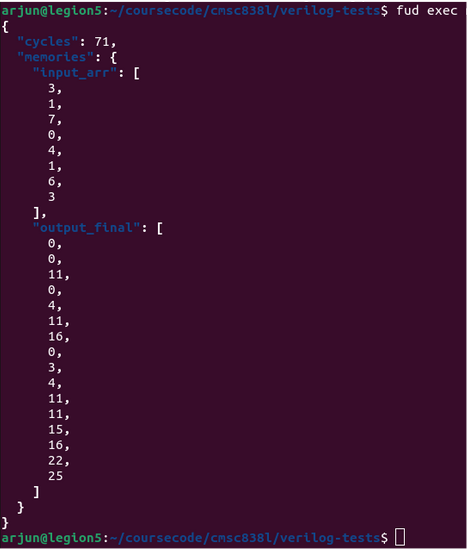
\includegraphics[height=25em]{images/prefix_sums.png}
    \caption{For running scan with an addition operator on 8 integers, we're getting 71 cycles, mostly because the speedup
    is limited by accessing the combinational memories (which takes at least a cycle) and because
    of the span-dependent "sweep-down" phase of the algorithm.}
\end{figure}
\subsection{Sequential scan}
As a comparison point, I also wrote a sequential version of scan, also in the Calyx IR. Due to the reduced dependence on
reading from and writing to combinational memories, the sequential version actually ran faster than the parallel implementation
(for n = 8).

\begin{figure}[H]
    \centering
    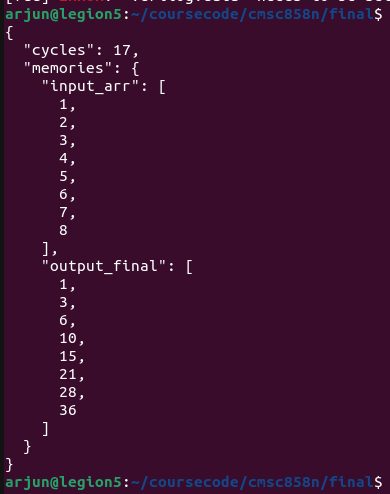
\includegraphics[height=25em]{images/seq_sums_scan.png}
    \caption{For the equivalent sequential version of scan, we get away with just 17 cycles. This is because the number of
    reads/writes to combinational memories is reduced by only having one register/value to deal with at a time. }
\end{figure}

\subsection{Filament HDL}
The Calyx IR is typically used with a frontend of some kind - in this case, the authors developed the Filament HDL, which
implements "timeline types" that allow hardware designers to reason about circuit propagation delays at the type system level.
This allows for compile time checks that can eliminate timing hazards between different parts of the circuit.

\subsubsection{Filament ALU}
To start, I first began by implementing an arithmetic logic unit in Filament, per the language documentation. This ALU is pipelined,
and allows the end-user to supply values that are added together concurrently by the ALU. This effectively solved the first step of
prefix sums, where each pair of elements is added together.

\begin{figure}[H]
    \centering
    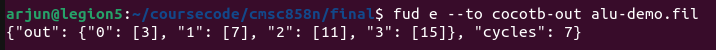
\includegraphics[width=\linewidth]{images/alu_result.png}
    \caption{The result of the pipelined ALU - even though we have 8 values (4 pairs) being added together, we're able to complete the
    work in just 7 cycles.}
\end{figure}

Following this, I wanted to start building part of the prefix sums tree (the "sweep-up" segment). However, even though Filament gives
relatively fine grained precision, I have been running into issues with persisting the results of each concurrent add so that they can be
propagated upwards. I have attempted to solve this with placing an additional register to persist the addition result, as well as using a
shift register (found in the Filament standard library) to capture the results of each addition operation, but the register appears to keep the
same result from the last addition operation instead of using the new result in the next step.

\begin{figure}[H]
    \centering
    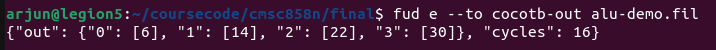
\includegraphics[width=\linewidth]{images/alu_result_doubled.png}
    \caption{The result of attempting to construct the next layer of the prefix sums tree - the circuit is retaining the same value in
    the storage register, instead of adding it to the result of the new addition operation.}
\end{figure}

As of 2024-05-17, I am still working on trying to resolve this issue to make more progress in the pipelined/parallelized version of
the prefix sums algorithm.
\end{document}